\textit{Google’s IDE Android Studio 2.1.2 was used for the implementation of the Android app prototype targeting Android 6.0 Marshmallow (\gls{API} level 23).}

\section{Stitch symbols}
There are different ways to display a stitch symbol in an Android app --- this section will give an overview of the possibilities and the solution chosen for the prototype. 
Since the \code{View} class already defines a canvas object with dedicated functions for drawing image and text content in its \code{onDraw()} method, it offers a good starting point. To decide between using the image or text format for displaying stitch symbols, a further look into what each format entails is necessary.

Image content needs to be specified in an Android project in the res directory under the drawable directory. This directory contains the image resources of the app, the drawables --- this applies for icons, custom images, and other image content, except for the launcher icon of the app, which is located in the mipmap directory. One way to use stitch symbols in an Android app would be to add every symbol as a drawable resource, and then draw those resources to the canvas of a view. For this a drawable would be needed for each individual stitch symbol, as well as way to map these drawable files to values that can be efficiently stored in a \gls{json} file. The usage of many drawables in an app would also lead to an increase in app size, resulting in longer download times and larger storage demands. Both are an inconvenience to the user and can be problematic on older devices with less powerful hardware, making the app unusable in the worst case scenario.
The other option for displaying symbols is to create a custom \gls{TTF} with glyphs for stitch symbols that is applied to text in the app. This is the solution used in the prototype. It offers several advantages over using image resources. For one, when using drawables it might be necessary to include several versions of the same file to ensure that they are displayed correctly on devices with different screen densities (\cite{android_screen_densities}). This is not needed for text with a custom font: the glyphs are defined by Beziér curves, which are correctly rendered by the system for the individual screen densities. The usage of a font also allows to write each stitch as a character, simplifying the process of saving a pattern to a \gls{json} file. For OpenType fonts, which \gls{TTF} belongs to, Microsoft recommends 64000 as the maximum number of glyphs a font should contain (\cite{microsoft_max_glyphs}). This allows for a plethora of stitch symbols. There are several knitting fonts available online, e.g. the Kauri Knits font by \cite{kauri} and the Knitter's Symbol font by \cite{xenakis}. To ensure that the knitting symbol glyphs fit within the style of the grid and row format an example of a custom knitting font was created for this thesis by the author.

The open source program FontForge \footnote{\url{https://fontforge.github.io/en-US/} (last accessed: 08-10-2016)} was used creation of the custom \gls{TTF} knitting font used in the prototype. The knitting font contains a selection of 16 stitch symbols whose glyphs were defined by the author herself. The glyphs and their corresponding UTF-8 characters can seen in \reffigure{fig:own_knitting_font}. The available symbols the knitting font offers as well as the corresponding symbol descriptions need to be defined as string arrays in the Constants class in the project.

\begin{figure}[H]
  \centering
  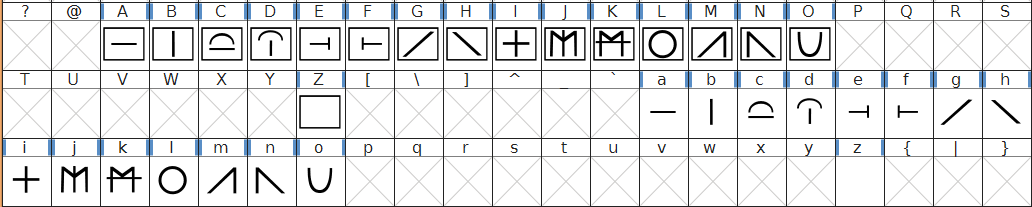
\includegraphics[width=.7\textwidth]{images/OwnKnittingFont_Chart.png}
  \caption[The custom knitting font used in the prototype \protect\newline{\small (own image)}]{The custom knitting font used in the prototype} 
  \label{fig:own_knitting_font} 
\end{figure}

\section{Pattern and Parsing between Pattern Formats}
Using a custom font for the stitch symbols allows for presenting patterns as a combinations of characters. The actual pattern chart is saved to a \gls{json} file as an \code{Array} of strings, where each string represents one row in the chart. For this a \code{Pattern} \gls{pojo} is used. It contains fields for the number of columns and rows, the current row set in the counter, and an array of strings, where each string represents a row in the pattern. A \code{Pattern} object’s default state after initialization contains a pattern of the size 10 x 10  cells that is filled with the string representing an empty stitch --- an empty stitch is represented by ``Z''in the prototype. The class \code{Pattern} is a subclass of \code{Metadata.java}, a class containing fields for a pattern name and a \gls{uuid}. More about the \code{Metadata} class can be found in Section \ref{implementation_storage}.

The actual pattern chart in the \code{Pattern} \gls{pojo} is saved in the shortened row notation. To display the pattern in the grid and row format, the pattern needs to be parsed into forms that are usable by both formats. For that the class \code{PatternParser.java} is used. It converts between the array of strings used in the Pattern \gls{pojo}, a two-dimensional \code{Array} of strings used in the \code{PatternGridView} (see Section \ref{impl_grid_format}), and a single string with linefeeds used in the row format's \code{EditText} widget (see Section \ref{impl_row_format}). For a more detailed explanation of the pattern notation forms refer to the corresponding sections.

\section{Persistent Disk Storage}
\label{implementation_storage}
There are multiple ways persistent storage can be implemented in Android. A common choice is to use a \code{SQLite} database, which Android natively supports (\cite{android_saving_data}). Another choice is to save data in files. The prototype implements the latter, since it reduces the export of files to a simple matter of copying to a different directory. Therefore, instead of using a database, the prototype saves \gls{json} files to the disk. This file type was chosen for the ease with which data can be saved and retrieved from the \gls{json} file. Files can be saved either to internal or external storage, as explained in \ref{android_storage}. Since permanent accessibility of files cannot be ensured for files located on the external storage, the pattern files are saved to internal storage, in the default directory that Android allocates for the app. When exporting they are copied to a directory on the user-accessible external storage. 

For this a \code{Pattern} \gls{pojo} is serialized using Google’s \gls{json} library \code{Gson}\footnote{\url{https://github.com/google/gson} (last accessed: 2016-08-09)}, which handles the marshalling and unmarshalling of the files to Java objects and vice versa. \code{Gson} supports the usage of Java generics and can map \gls{json} data to \gls{pojo}s while maintaining inheritance hierarchies. The corresponding code can be in found the class \code{PatternStorage.java} (see Appendix \ref{code:patternstorage}).

The \code{Pattern} class inherits from the class \code{Metadata} which contains both a \gls{uuid} which is used as a pattern's file name and the pattern name that is given by the user. When storing on disk, \code{Pattern} \gls{pojo}s are converted to \gls{json} using \code{Gson} and saved with the \gls{uuid} as filename to avoid collisions in file names. Before that the metadata of the pattern is added to a local \code{ArrayList} of \code{Metadatas} in the \code{PatternStorage class}.  This \code{ArrayList} in turn is marshalled to \gls{json} and saved to the same directory as the pattern files. It acts as an index of all patterns saved on the device. Using this index file increases performance, since not all pattern files, with their potentially big pattern data, have to be accessed and unmarshalled --- instead only the lightweight metadata files need to be loaded. Individual patterns can then be loaded using the \gls{uuid} saved in the patterns \code{Metadata}.

\section{Displaying a Pattern}

\subsection{Grid Format}
\label{impl_grid_format}
When considering presenting data in a grid format, the most obvious solution is to first look at Android's own implementations of grids. Promising starting points for that are the \code{TableLayout} and the \code{GridView} class. After a brief investigation into the \code{TableLayout}, it quickly becomes apparent, that this layout is intended more as a way to position views, than to represent data in a grid. It can be likened to the \code{HTML} table tag (\cite{android_tablelayout}), which is also used to position views within the constraints of cells, columns, and rows.

Android's code class, on the other hand, is designed with notion of displaying data. Each cell represents one data entry in a collection of data, the displaying of which is handled by an Adapter class attached to the grid view. Android ships with a specialized adapter for lists \footnote{\url{https://developer.android.com/reference/android/widget/ListAdapter.html} (accessed: 11-08-2016)}, as well as a \code{BaseAdapter} that can be subclassed for a custom handling and presentation of data. While this is a fitting solution for displaying symbols in a grid, it does not meet the requirements this project sets for the grid format. It is required that the column and row numbers are displayed next to the grid as axes. These axes should scale and scroll together with the grid, but should not be scrolled outside the visible area, since the user would not be able to know the cell position then. For one, the \code{GridView} class does not support frozen cells, columns, or rows --- as far as the author of this thesis was able to research. If the column numbers were to be displayed in the first row of the grid, they would move offscreen upon scrolling the grid. A possible solution to this would to use text views to act as axes to the grid and to display the column and row numbers next to it. Problematic with this approach would be the fine-tuning required to match the visuals of the text view to that of the grid. Line height, text size and the synchronization with scrolls and zooms performed on the grid would need to match perfectly. Since this does not classify as intended behavior for these views, a cohesive \gls{UI} cannot be guaranteed. Furthermore, Android does not offer two dimensional scroll on any view except its WebView\footnote{\url{https://developer.android.com/reference/android/webkit/WebView.html} (accessed: 11-08-2016)} -- the GridView class natively only supports vertical scroll.

Therefore, in order to fulfill all requirements it makes the most sense to create a custom implementation of a view that supports the display of text in a grid, two-dimensional scroll, zoom, and axes that stick to the view bounds. Google's sample project \textit{Interactive Chart}\footnote{\url{https://developer.android.com/shareables/training/InteractiveChart.zip} (accessed: 11-08-2016) A digital copy of this project can also be found on the CD attached to this thesis.} and the corresponding training path\footnote{\url{https://developer.android.com/training/gestures/scale.html##drag} (accessed: 11-08-2016)} present an implementation example and were used as a guideline for the implementation of the class \code{PatternGridView.java} (see Appendix \ref{code:patterngridview}). This class keeps a reference to a two-dimensional array of strings which represents the pattern with its columns and rows. The grid and its axes are drawn by overriding the \code{onDraw()} method, calculating the position of the corresponding lines and numbers with the dimensions of the view and predefined, hardcoded values for cell width and margin. The current version of the \code{PatternGridView} uses a \code{SimpleOnGestureListener}\footnote{\url{https://developer.android.com/reference/android/view/GestureDetector.SimpleOnGestureListener.html} (last accessed: 2016-08-11)} to compute two-dimensional dragging. Android defines two different scrolling types for views: dragging and flinging (\cite{android_scrolling_types}). Dragging is executed by dragging a finger across the device's touchscreen and results in a moving of the view corresponding to the dragging direction and speed. This means, that no matter the velocity of the dragging gesture, the view will not keep moving once the user lifts the finger involved in the gesture. A fling will keep moving the view with a speed and duration exponential to the velocity of the fling gesture, where the duration is calculated by introducing a friction to the scroll. This gesture can also be describe as a swiping motion performed on the touchscreen. Even after the finger has been lifted of the screen the fling continues to execute until it either runs its course or is interrupted.

The current version of the \code{PatternGridView} implements a simple dragging gesture and does not support flinging as of yet. For this a variable of type \code{PointF}\footnote{\url{https://developer.android.com/reference/android/graphics/PointF.html} (last accessed: 2016-08-11)} is saved locally to represent the offset scrolled. It is initialized with the value (0,0) and updated on every motion event that is recognized as dragging. The necessary calculations for these updates are done by overriding the \code{onScroll()} method in a custom \code{SimpleOnGestureListener}. This method has access to the horizontal and vertical distance scrolled, which is subtracted from the offset. This is done because the value of the distance is positive when dragging towards the point of origin (the top left corner) and negative when dragging away from it. Therefore, the canvas needs to be translated in the opposite distance. The offset is then clamped to minimum and maximum values, to ensure that the grid will never completely move offscreen: 

\begin{gather*}
offset_{min} = (0, 0)
\end{gather*}
\begin{align*}
offset_{max} = (&width_{view} - width_{content} - 2 * margin, \\
				&height_{view} - height_{content} - 2 * margin)
\end{align*}

where margin is the distance of the grid from the top and left view edges that is reserved for the axes text.

Similarly to dragging, scaling is implemented with a \code{SimpleOnScaleGestureListener}\footnote{\url{https://developer.android.com/reference/android/view/ScaleGestureDetector.SimpleOnScaleGestureListener.html} (last accessed: 2016-08-11)} with is connected to the view's \code{onTouchEvent()}. The scaling factor is then clamped at pre-defined maximum and minimum values and saved in a variable. The scale factor is then used during the drawing operation to scale the gridlines, axes, and test. When touching the grid the touched cell is calculated from the pixel position of the touch event. The currently selected stitch string is then saved to that position in the two-dimensional pattern array. Following this the view is invalidated\footnote{\url{https://developer.android.com/reference/android/view/View.html##invalidate()} (last accessed 2016-08-11)} and redrawn with the updated pattern.   

\subsection{Row Format}
\label{impl_row_format}
The row editor should display line numbers at the left side of the screen and keep them in that position during horizontal scrolling, so that they will not move offscreen. Additionally, it should support the standard text editor functions: text select, copy, cut, and paste. It should display text in multiple lines that do not wrap at the end of the screen, but continue offscreen until a newline is input and the content needs to be scrollable horizontally and vertically. Android's \code{EditText} widget\footnote{\url{https://developer.android.com/reference/android/widget/EditText.html}} fulfills most of these requirements. The \code{EditText} widget inherits from the class \code{EditText} which is specialised for displaying text content. It supports standard text editing functions, can display multiple lines of text, and supports vertical scrolling. Unfortunately, it does not natively support text lines to continue offscreen --- upon reaching the width of the widget the text is wrapped to the next line. Another problem is, that the widget always automatically triggers the showing of Android's on-screen keyboard when it receives focus, i.e. when the user taps the view to start text input. 

One instance, when the on-screen keyboard, also called the soft input method (\cite{android_softinputmethod}), is shown, is when the activity's main windows has input focus (\cite{android_windowsoftinputmode_docs}). An activity receives input focus on activity start and resume when containing an \code{EditText} widget in its view hierarchy. This behavior can be suppressed by declaring the state of the soft input method in the manifest file (see Appendix \ref{code:manifest}) of the project as hidden (see \reflisting{lst:inputstate_hidden_manifest}).

\begin{lstlisting}[language=JAVA, caption=Declaring on-screen keyboard hidden in manifest file., label=lst:inputstate_hidden_manifest]
	...
	<activity android:name=".EditorActivity"
	            android:windowSoftInputMode="stateAlwaysHidden"/>
	...
\end{lstlisting}

Interaction with an \code{EditText} widget will also show the on-screen keyboard: the widget's \code{onClick()} and \code{onLongClick()} listeners trigger the soft input method. To avoid this the custom widget \code{KeyboardlessEditText}\footnote{\url{https://github.com/danialgoodwin/android-widget-keyboardless-edittext}}, written by Danial Goodwin, is used in the prototype. It offers the the same functions as a native Android \code{EditText} widget, but will suppress the showing of the on-screen keyboard.

To improve the visibility of the lines the \code{LinedEditor} (see Appendix \ref{code:linededitoredittext}) class is subclassed from the keyboardless \code{EditText} widget and a background is drawn behind every other line. The \code{LinedEditor} is part of the \code{RowEditorLinearLayout} (see Appendix \ref{code:roweditorlinearlayout}), a custom \code{LinearLayout} which houses the complete row format editing functionality. This layout will be referred to as the row editor. A \code{LineNumberTextView} (see Appendix \ref{code:linenumbertextview}), a custom \code{TextView}, is placed to the left of the \code{LinedEditor} and displays the line numbers. To achieve a consistent look of both line numbers and editor text the same font and text size are set on both \code{EditText} and \code{EditText} widget.
To suppress the \code{EditText} widget's line wrap behavior its width is set to the value \textit{wrap\char`_content} (see \reflisting{lst:row_editor_xml}). This allows the widget to increase its width when text is added that exceeds the current width of the view.

\begin{lstlisting}[
		language=XML, 
		caption=Excerpt from row\char`_editor.xml, 
		label=lst:row_editor_xml
	]
	...
    <de.muffinworks.knittingapp.views.LinedEditorEditText
    android:paddingRight="50dp"
    style="@style/DisplayEditTextStyle"
    android:id="@+id/row_editor_edit_text"
    android:gravity="center_vertical|left"
    android:textSize="@dimen/row_editor_default_text_size"
    android:layout_width="wrap_content"
    android:layout_height="wrap_content"/>
	...
\end{lstlisting}

The \code{LinedEditor}'s parent layout has a \code{Scroller}\footnote{\url{https://developer.android.com/reference/android/widget/Scroller.html}} object attached to it which it used to scroll its children. The calculations needed for the scrolling behavior of the parent layout were adapted from the class \code{TwoDScrollView}, written by \cite{clark2010}. 

The row editor in the current version of the prototype does not completely fulfill all requirements. On row editor instantiation the editor requests the \code{LinedEditor}'s dimensions and line count before the widget has been completely built. This results in a line count return value of zero, no matter how many lines of text have been set in the widget initially. The line numbers in the row editor then display the lowest line number possible: one. Additionally, the parent layout is not able to enable scrolling for offscreen text content, since the child measurements are incorrect. This could be solved by requesting the \code{EditText} widget's dimensions at a later time when all views and layouts have been built. At the time of writing the author has not determined the correct timing yet. More research into the lifecycle of the widget is required.

Additionally, the timing of measurements are also the cause for the another issue. Upon adding a new line which would lie outside of the visible area, the row editor should scroll the new line into view. Instead only the line above the new line is scrolled into view. This might be caused by measuring the \code{EditText} widget before its height is updated to include the height of the new line. To determine a solution to this further research is needed.

The \code{EditText} widget also returns the wrong position when more text is added at the end of a line. Instead of calculating the cursor's new position by increasing the value of its x-coordinates by the width of added text, the returned position is located at the first character of the next line. This might be due to the suppressed line wrapping behavior of \code{EditText} widget in multi-line mode. Despite returning an incorrect cursor position upon text change, the text and cursor are displayed at the correct location and not wrapped to the following line. This presents a problem when scrolling to offscreen text changes at the of a line. Instead of scrolling to the end of the edited line, the scroll will move the beginning of the next line into view.

Lastly, the line numbers do not stay visible when the row editor is scrolled horizontally which reduces its usability since the user cannot at all times tell the line number of a row. This behavior might be achieved by attaching different scrollers to the \code{EditText} for the line numbers and the \code{EditText} widget, but the time constraints of this thesis did not allow further research. 

\section{Keyboard}
The row and the grid editor each use different symbol keyboards. The keys of the grid editor keyboard feature stitch symbols and a delete button. Keys can be toggled to an active state --- only one key at a time can be active. While a key is active, touching the grid will lead to the string corresponding with the active key being added to the pattern at the location of the touched cell. Since empty cells contain the designated empty character ``Z'', deletion works in the same way as setting a symbol on the grid. The keyboard is implemented using a \code{Gridview}\footnote{\url{https://developer.android.com/reference/android/widget/GridView.html}}, a default Android component to display a collection of items in a grid with equal spacing between all items. The gridview also by default supports vertical scrolling. A grid item consists of text set on a button of the class \code{KnittingFontButton}, a custom class extending Android’s own \code{Button} widget. The custom button sets the knitting font to display its string title as a knitting symbol. Set on the button are a click listener and a long click listener. The click listener toggles the state of the key and on long click the description of the symbol displayed on the button is shown at the bottom of the screen.

In the row editor the keyboard is divided in three sections. One section contains the stitch symbols, one a number pad and one an enter and a backspace button. Pressing a key on either number pad or symbols section appends the corresponding string or number to the editor at the current position of the cursor. The enter and backspace button call the system’s enter and backspace key events from Android’s software keyboard and do therefore not require custom handling, but only to be forwarded to the editor.

The symbols sections is also a Gridview, although with less columns than in the grid editor. The numpad uses the \code{CalculatorPadLayout} from the Android Open Source Project's Calculator project project\footnote{\url{https://android.googlesource.com/platform/packages/apps/Calculator/+/refs/tags/android-6.0.1_r7/src/com/android/calculator2/CalculatorPadLayout.java}}. The \code{CalculatorPadLayout} takes a number of child views, in this case \code{KnittingFontButtons}, as well as arguments for row and column count. It then calculates the size of the child views, so that all are equal in size. This custom layout is used because it optimally arranges its children in the available space without scrolling. A \code{Gridview}, on the other hand, is built to dynamically accommodate data and possible data changes --- it is only concerned with the number of columns the data views can be placed in, if the \code{Gridview} bounds are too small to display all rows they will automatically placed offscreen and the \code{Gridview} will become scrollable --- an undesired and atypical behaviour for a number pad, in the author's opinion.

\section{Viewer with Row Counter}
The row counter and the viewer are implemented in the \code{ViewerActivity} class (see Appendix \ref{code:vieweractivity}). The activity's layout file defines a container \code{FrameLayout}\footnote{\url{https://developer.android.com/reference/android/widget/FrameLayout.html}} for the pattern content and below that the row counter \gls{UI}. On its creation the activity instantiates a \code{PatternGridView} and a \code{RowEditorLinearLayout} and sets the data of the viewed pattern on both. The view and the layout can then be switched out at runtime inside their container by adding and removing the required view whenever the user decides to switch between grid and row format.
At the current version of the prototype the row format is still experiencing some issues: the line numbers are not correctly instantiated and the pattern, if larger than the screen, is not scrollable inside the viewer.

The row counter below the pattern features a display the current row number the user is at in the knitting pattern and two buttons: one for increasing the counter and one for decreasing. The current row is set on both pattern format views as well, but only indicated with a visual highlight in the grid format. The grid format also scrolls the current row into view whenever an increase or decrease happens and the current row is offscreen. 

The ActionBar contains the following action buttons

\begin{itemize}
\item Switch pattern formats
\item Open glossary
\item Scroll to current row
\item Export pattern
\item Reset row counter
\item Edit pattern
\end{itemize}

where the last three buttons are located in the overflow section.

\section{Editor}
The class \code{EditorActivity.java} (see Appendix \ref{code:editoractivity}) contains, just like the \code{ViewerActivity}, a \code{FrameLayout} to programmatically add the grid and row editor fragments to and allow easy switching between the visible fragments. The ActionBar contains the following action buttons 

\begin{itemize}
\item Switch pattern editor formats
\item Save
\item Set grid size
\item Export pattern
\item open glossary
\item Edit pattern name
\item Delete pattern
\end{itemize}

where the last four buttons can be found in the overflow section. The action button to set the grid size is only shown when the pattern is being edited in the grid format.

Upon switching the pattern formats changes to the pattern are automatically saved and upon success a short message is shown to the user. When the user tries to exit the editor while there are still unsaved changes a dialog is shown, offering to save the changes or to discard them and close the editor. After a pattern is exported an info dialog displays the directory on the external storage that the file was exported to.
The activity also handles the showing of dialog fragments to request user input and processes the results. The dialogs handled in the \code{EditorActivity} are the \code{GridSizeDialogFragment} (see Appendix \ref{code:gridsizedialogfragment}), the \code{PatternDeleteDialogFragment} (see Appendix \ref{code:patterndeletedialogfragment}), and the \code{PatternNameDialogFragment} (see Appendix \ref{code:patternnamedialogfragment}).

\addcontentsline{toc}{subsection}{Editor Fragments}
\subsection*{Editor Fragments}
Each of the two editor formats has its own fragment that displays the appropriate keyboard for the selected format. The fragments handle the saving, loading, and updating of the pattern data as well as the keyboard events. The grid format fragment also displays the dialog for changing the grid size.

\section{Pattern List}
The prototype launches with the \code{PatternListActivity} (see Appendix \ref{code:patternlistactivity}) that displays all files currently indexed in the \code{Metadata} file (see section \ref{implementation_storage}). For that Android's \code{ListView}\footnote{\url{https://developer.android.com/reference/android/widget/ListView.html} \label{url_footnote}} component is used. For each file the pattern name, a button to edit (pencil icon), and a button to delete (trashcan icon) the pattern are shown. The edit button opens the selected pattern in the \code{EditorActivity} and upon delete the \code{PatternDeleteDialogFragment} is shown.

\section{Glossary}
Like the \code{PatternListActivity}, the \code{GlossaryActivity} also uses a \code{ListView}\footnote{see footnote \ref{url_footnote}} to display the symbols and their descriptions. The symbols and their descriptions are taken from the \code{Constants} class.

\begin{figure}[H]
	\centering
	\begin{subfigure}[b]{0.5\textwidth}
	  \centering
	    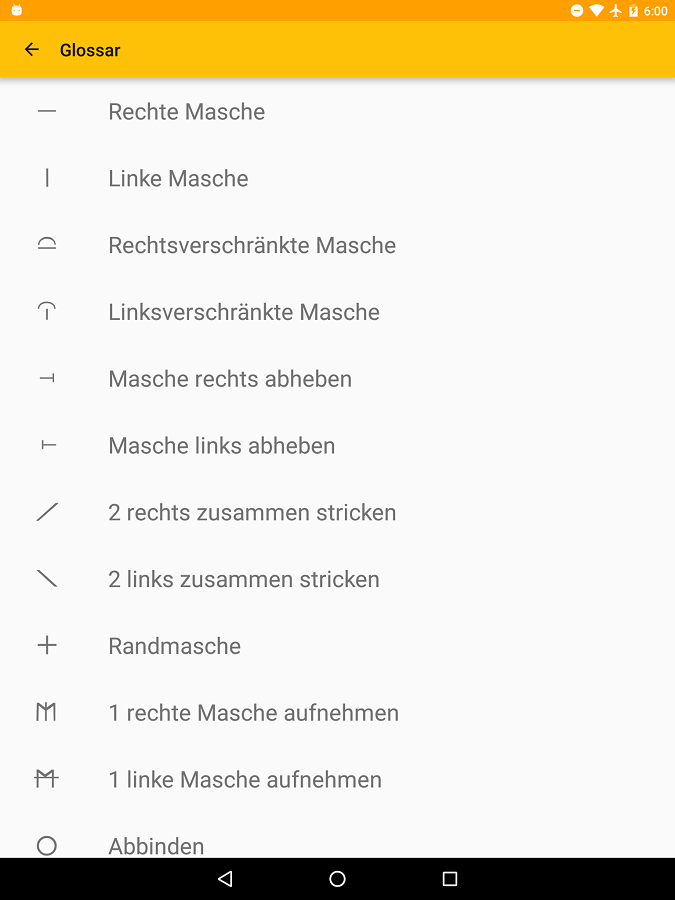
\includegraphics[width=0.95\linewidth]{images/glossary_h900.png}
	    \caption[The glossary \protect\newline{\small (own image)}]{The glossary}
	  \label{fig:glossary}
	\end{subfigure}
	\begin{subfigure}[b]{0.5\textwidth}
	  \centering
	    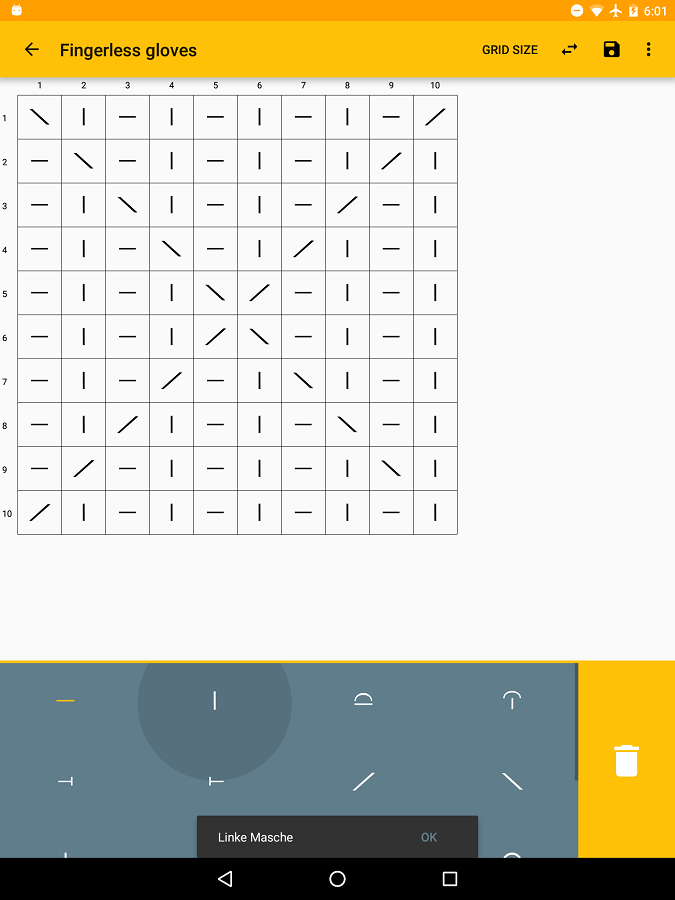
\includegraphics[width=0.95\linewidth]{images/keyboard_symbol_description_h900.png}
	    \caption[The grid editor while showing a symbol description \protect\newline{\small (own image)}]{The grid editor while showing a symbol description}
	    \label{fig:editor}
	\end{subfigure}
	\caption{Screenshots of the current version of the prototype}
\end{figure}

\begin{figure}[H]
	\centering
	\begin{subfigure}[b]{0.5\textwidth}
	  \centering
	    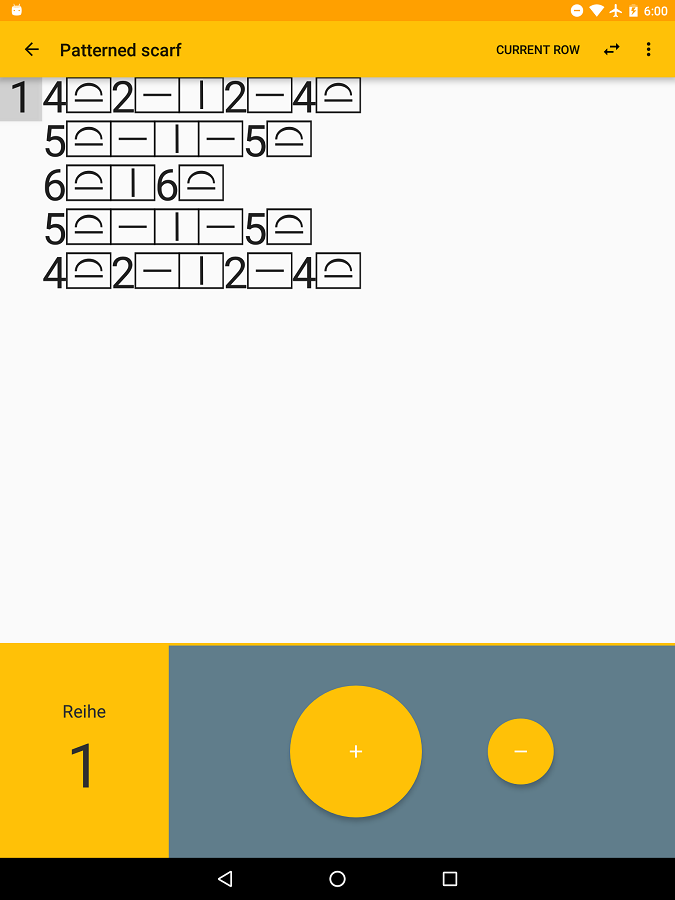
\includegraphics[width=0.95\linewidth]{images/viewer_row_h900.png}
	    \caption[The viewer \protect\newline{\small (own image)}]{The viewer}
	  \label{fig:viewer}
	\end{subfigure}
	\begin{subfigure}[b]{0.5\textwidth}
	  \centering
	    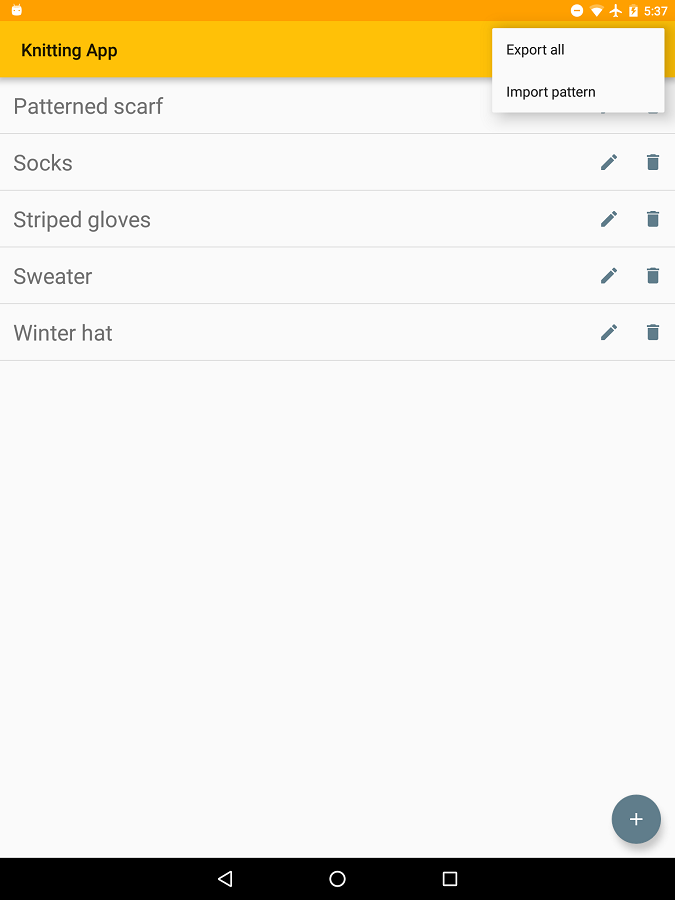
\includegraphics[width=0.95\linewidth]{images/pattern_list_open_menu_h900.png}
	    \caption[The list of stored patterns \protect\newline{\small (own image)}]{The list of stored patterns}
	  \label{fig:patternlist}
	\end{subfigure}
	\caption{Screenshots of the current version of the prototype}
\end{figure}